
%(BEGIN_QUESTION)
% Copyright 2015, Tony R. Kuphaldt, released under the Creative Commons Attribution License (v 1.0)
% This means you may do almost anything with this work of mine, so long as you give me proper credit

Read selected portions of the Siemens ``SIMATIC S7-200 Programmable Controller System Manual'' (document A5E00307987-04, August 2008) and answer the following questions:

\vskip 10pt

Identify the different types of SIMATIC {\it counter} instructions.

\vskip 10pt

Identify a practical application for a counter instruction programmed into a PLC.

\vskip 10pt

How high can one of these counter instructions count up to?  How low can it count down to?  Based on these values, how many bits do you think are used in the register to store a counter instruction's current value?

\vskip 10pt

Sketch a simple ladder-diagram program for a Siemens S7-200 PLC whereby a switch connected to input {\tt I0.5} causes a counter to increment (count {\it up}) and then turn on an alarm light output {\tt Q0.3} when the count reaches a value of 5.  Also provide a ``reset'' function triggered by a normally-open switch contact at input {\tt I0.0} to force the count value back to zero when pressed.

\vskip 20pt \vbox{\hrule \hbox{\strut \vrule{} {\bf Suggestions for Socratic discussion} \vrule} \hrule}

\begin{itemize}
\item{} If you have access to your own PLC for experimentation, I urge you to write a simple {\it demonstration} program in your PLC allowing you to explore the behavior of these PLC instructions.  The program doesn't have to do anything useful, but merely demonstrate what each instruction does.  First, read the appropriate section in your PLC's manual or instruction reference to identify the proper syntax for that instruction (e.g. which types of data it uses, what address ranges are appropriate), then write the simplest program you can think of to demonstrate that function in isolation.  Download this program to your PLC, then run it and observe how it functions ``live'' by noting the color highlighting in your editing program's display and/or the numerical values manipulated by each instruction.  After ``playing'' with your demonstration program and observing its behavior, write comments for each rung of your program explaining in your own words what each instruction does.
\end{itemize}

\underbar{file i02245}
%(END_QUESTION)





%(BEGIN_ANSWER)

\noindent
{\bf Partial answer:}

\vskip 10pt

Each of the S7-200 counter instructions can count as high as +32767 and as low as $-32768$.  This equates to 16 bits, signed integer (2's complement notation, where the MSB has a negative place-weight value of $-32768$).

%(END_ANSWER)





%(BEGIN_NOTES)

Three types of SIMATIC counter instructions: count up (CTU), count down (CTD), and count up/down (CTUD).

\vskip 10pt

Practical uses include counting objects on an assembly line, counting number of times a machine has been started or shut down, or counting any other sort of discrete event(s).

\vskip 10pt

Each of the S7-200 counter instructions can count as high as +32767 and as low as $-32768$.  This equates to 16 bits, signed integer (2's complement notation, where the MSB has a negative place-weight value of $-32768$).

\vskip 10pt

Simple counter program to fulfill stated requirements:

$$\includegraphics[width=15.5cm]{i02245x01.eps}$$

%INDEX% Reading assignment: Siemens S7-200 system manual (counter instructions)

%(END_NOTES)


